\documentclass[10pt,journal,compsoc,onecolumn]{IEEEtran}

\usepackage[T1]{fontenc}
\usepackage{amsmath,amssymb}
\usepackage{graphicx}
\usepackage{booktabs}
\usepackage{xcolor}
\usepackage[sc]{mathpazo}
\usepackage[varqu,scaled=0.95]{inconsolata}
\usepackage{microtype}
\usepackage[hidelinks]{hyperref}

% a table wider than the text block is scaled down to it
\newsavebox{\fitbox}
\newenvironment{fit}{\begin{lrbox}{\fitbox}}{\end{lrbox}%
  \ifdim\wd\fitbox>\linewidth\resizebox{\linewidth}{!}{\usebox{\fitbox}}\else\usebox{\fitbox}\fi}
\graphicspath{{gen/figures/}}
\newcommand{\arm}[1]{\texttt{#1}}
\newcommand{\eps}{\varepsilon}
\makeatletter\newcommand{\gen}[1]{\@@input gen/#1.tex }\makeatother
\renewcommand{\IEEEcompsocdiamondline}{}
% generated by mvs.paper; do not edit
\newcommand{\warmPasses}{20}
\newcommand{\rewarmSteps}{100}
\newcommand{\horizon}{300}
\newcommand{\evalEvery}{10}
\newcommand{\evalSamples}{512}
\newcommand{\maxSteps}{2000}
\newcommand{\warmupSteps}{100}
\newcommand{\bootDraws}{10000}
\newcommand{\nCells}{540}
\newcommand{\nArms}{15}
\newcommand{\nSeedsMin}{3}
\newcommand{\nSeedsMax}{3}
\newcommand{\seedsXS}{3}
\newcommand{\paramsXS}{0.8}
\newcommand{\seedsS}{3}
\newcommand{\paramsS}{10.7}
\newcommand{\seedsM}{3}
\newcommand{\paramsM}{25.3}
\newcommand{\epsMin}{10.0}
\newcommand{\epsMax}{36.2}
\newcommand{\bandLamMin}{4}
\newcommand{\bandLamMax}{216}
\newcommand{\payFull}{100}
\newcommand{\peakFull}{0.0}
\newcommand{\ratioFull}{0.00}
\newcommand{\lamFull}{0.0}
\newcommand{\regretFull}{0.00}
\newcommand{\inbandFull}{12/12}
\newcommand{\censFull}{0}
\newcommand{\lateFull}{--}
\newcommand{\payWMqeightVlogeight}{50}
\newcommand{\peakWMqeightVlogeight}{2.2}
\newcommand{\ratioWMqeightVlogeight}{0.09}
\newcommand{\lamWMqeightVlogeight}{1.1}
\newcommand{\regretWMqeightVlogeight}{0.12}
\newcommand{\inbandWMqeightVlogeight}{12/12}
\newcommand{\censWMqeightVlogeight}{0}
\newcommand{\lateWMqeightVlogeight}{--}
\newcommand{\payWMVrone}{67}
\newcommand{\peakWMVrone}{4.1}
\newcommand{\ratioWMVrone}{0.17}
\newcommand{\lamWMVrone}{4.4}
\newcommand{\regretWMVrone}{0.23}
\newcommand{\inbandWMVrone}{12/12}
\newcommand{\censWMVrone}{0}
\newcommand{\lateWMVrone}{--}
\newcommand{\payWV}{67}
\newcommand{\peakWV}{6.8}
\newcommand{\ratioWV}{0.29}
\newcommand{\lamWV}{8.2}
\newcommand{\regretWV}{0.72}
\newcommand{\inbandWV}{12/12}
\newcommand{\censWV}{0}
\newcommand{\lateWV}{--}
\newcommand{\payWVsvdfour}{34}
\newcommand{\peakWVsvdfour}{7.9}
\newcommand{\ratioWVsvdfour}{0.33}
\newcommand{\lamWVsvdfour}{8.7}
\newcommand{\regretWVsvdfour}{0.80}
\newcommand{\inbandWVsvdfour}{12/12}
\newcommand{\censWVsvdfour}{0}
\newcommand{\lateWVsvdfour}{--}
\newcommand{\payWEmbV}{34}
\newcommand{\peakWEmbV}{7.4}
\newcommand{\ratioWEmbV}{0.31}
\newcommand{\lamWEmbV}{8.9}
\newcommand{\regretWEmbV}{0.82}
\newcommand{\inbandWEmbV}{12/12}
\newcommand{\censWEmbV}{0}
\newcommand{\lateWEmbV}{--}
\newcommand{\payWVrone}{33}
\newcommand{\peakWVrone}{7.4}
\newcommand{\ratioWVrone}{0.31}
\newcommand{\lamWVrone}{9.1}
\newcommand{\regretWVrone}{0.80}
\newcommand{\inbandWVrone}{12/12}
\newcommand{\censWVrone}{0}
\newcommand{\lateWVrone}{--}
\newcommand{\payWbfsixteenVrone}{17}
\newcommand{\peakWbfsixteenVrone}{7.5}
\newcommand{\ratioWbfsixteenVrone}{0.31}
\newcommand{\lamWbfsixteenVrone}{9.1}
\newcommand{\regretWbfsixteenVrone}{0.85}
\newcommand{\inbandWbfsixteenVrone}{12/12}
\newcommand{\censWbfsixteenVrone}{0}
\newcommand{\lateWbfsixteenVrone}{--}
\newcommand{\payWM}{67}
\newcommand{\peakWM}{1469.1}
\newcommand{\ratioWM}{69.26}
\newcommand{\lamWM}{634.6}
\newcommand{\regretWM}{177.36}
\newcommand{\inbandWM}{0/12}
\newcommand{\censWM}{9}
\newcommand{\lateWM}{40}
\newcommand{\payWZero}{33}
\newcommand{\peakWZero}{271.3}
\newcommand{\ratioWZero}{11.40}
\newcommand{\lamWZero}{56.8}
\newcommand{\regretWZero}{19.80}
\newcommand{\inbandWZero}{3/12}
\newcommand{\censWZero}{3}
\newcommand{\lateWZero}{75}
\newcommand{\payWFresh}{33}
\newcommand{\peakWFresh}{105.7}
\newcommand{\ratioWFresh}{4.38}
\newcommand{\lamWFresh}{26.4}
\newcommand{\regretWFresh}{6.40}
\newcommand{\inbandWFresh}{5/12}
\newcommand{\censWFresh}{3}
\newcommand{\lateWFresh}{25}
\newcommand{\payWRewarm}{33}
\newcommand{\peakWRewarm}{19.8}
\newcommand{\ratioWRewarm}{0.83}
\newcommand{\lamWRewarm}{35.3}
\newcommand{\regretWRewarm}{2.88}
\newcommand{\inbandWRewarm}{11/12}
\newcommand{\censWRewarm}{1}
\newcommand{\lateWRewarm}{--}
\newcommand{\payWWarmv}{33}
\newcommand{\peakWWarmv}{9.5}
\newcommand{\ratioWWarmv}{0.40}
\newcommand{\lamWWarmv}{27.2}
\newcommand{\regretWWarmv}{0.68}
\newcommand{\inbandWWarmv}{10/12}
\newcommand{\censWWarmv}{0}
\newcommand{\lateWWarmv}{55}
\newcommand{\payWMWarm}{67}
\newcommand{\peakWMWarm}{13.1}
\newcommand{\ratioWMWarm}{0.55}
\newcommand{\lamWMWarm}{23.7}
\newcommand{\regretWMWarm}{0.40}
\newcommand{\inbandWMWarm}{9/12}
\newcommand{\censWMWarm}{0}
\newcommand{\lateWMWarm}{20}
\newcommand{\payWWarm}{33}
\newcommand{\peakWWarm}{204.0}
\newcommand{\ratioWWarm}{8.44}
\newcommand{\lamWWarm}{64.2}
\newcommand{\regretWWarm}{15.15}
\newcommand{\inbandWWarm}{4/12}
\newcommand{\censWWarm}{3}
\newcommand{\lateWWarm}{30}
\newcommand{\forkList}{200, 600, 1200, 1700}
\newcommand{\sizeQXS}{0.07}
\newcommand{\sizeVXS}{0.20}
\newcommand{\sizeRankXS}{0.22}
\newcommand{\sizeRankBfXS}{0.26}
\newcommand{\sizeMXS}{42.10}
\newcommand{\sizeZeroXS}{2.51}
\newcommand{\sizeFreshXS}{1.08}
\newcommand{\sizeRewarmXS}{0.71}
\newcommand{\sizeWarmvXS}{0.22}
\newcommand{\sizeWarmXS}{3.72}
\newcommand{\sizeQS}{0.02}
\newcommand{\sizeVS}{0.30}
\newcommand{\sizeRankS}{0.31}
\newcommand{\sizeRankBfS}{0.31}
\newcommand{\sizeMS}{102.63}
\newcommand{\sizeZeroS}{9.58}
\newcommand{\sizeFreshS}{4.11}
\newcommand{\sizeRewarmS}{0.89}
\newcommand{\sizeWarmvS}{0.34}
\newcommand{\sizeWarmS}{9.23}
\newcommand{\sizeQM}{0.09}
\newcommand{\sizeVM}{0.29}
\newcommand{\sizeRankM}{0.31}
\newcommand{\sizeRankBfM}{0.31}
\newcommand{\sizeMM}{69.26}
\newcommand{\sizeZeroM}{11.40}
\newcommand{\sizeFreshM}{4.38}
\newcommand{\sizeRewarmM}{0.83}
\newcommand{\sizeWarmvM}{0.40}
\newcommand{\sizeWarmM}{8.44}
\newcommand{\epsEarly}{24.8}
\newcommand{\peakEarlyQ}{6.1}
\newcommand{\ratioEarlyQ}{0.25}
\newcommand{\peakEarlyV}{18.5}
\newcommand{\ratioEarlyV}{0.75}
\newcommand{\peakEarlyRank}{21.6}
\newcommand{\ratioEarlyRank}{0.87}
\newcommand{\peakEarlyRankBf}{21.7}
\newcommand{\ratioEarlyRankBf}{0.88}
\newcommand{\peakEarlyM}{1539.2}
\newcommand{\ratioEarlyM}{62.14}
\newcommand{\peakEarlyZero}{750.1}
\newcommand{\ratioEarlyZero}{30.28}
\newcommand{\peakEarlyFresh}{347.9}
\newcommand{\ratioEarlyFresh}{14.04}
\newcommand{\peakEarlyRewarm}{56.9}
\newcommand{\ratioEarlyRewarm}{2.30}
\newcommand{\peakEarlyWarmv}{28.5}
\newcommand{\ratioEarlyWarmv}{1.15}
\newcommand{\peakEarlyWarm}{663.1}
\newcommand{\ratioEarlyWarm}{26.77}
\newcommand{\epsLate}{16.4}
\newcommand{\peakLateQ}{0.1}
\newcommand{\ratioLateQ}{0.01}
\newcommand{\peakLateV}{0.1}
\newcommand{\ratioLateV}{0.01}
\newcommand{\peakLateRank}{0.1}
\newcommand{\ratioLateRank}{0.01}
\newcommand{\peakLateRankBf}{0.2}
\newcommand{\ratioLateRankBf}{0.01}
\newcommand{\peakLateM}{214.5}
\newcommand{\ratioLateM}{13.05}
\newcommand{\peakLateZero}{9.3}
\newcommand{\ratioLateZero}{0.57}
\newcommand{\peakLateFresh}{2.0}
\newcommand{\ratioLateFresh}{0.12}
\newcommand{\peakLateRewarm}{1.5}
\newcommand{\ratioLateRewarm}{0.09}
\newcommand{\peakLateWarmv}{0.4}
\newcommand{\ratioLateWarmv}{0.02}
\newcommand{\peakLateWarm}{1.2}
\newcommand{\ratioLateWarm}{0.07}
\newcommand{\bytesWorstPct}{0.04}
\newcommand{\overshootA}{2.13}
\newcommand{\overshootAtA}{13}
\newcommand{\overshootB}{6.57}
\newcommand{\overshootAtB}{12}
\newcommand{\firstNoiseA}{4.4}
\newcommand{\excessZerosA}{109}
\newcommand{\firstNoiseB}{13.8}
\newcommand{\excessZerosB}{1292}
\newcommand{\firstNoiseC}{1.9}
\newcommand{\excessZerosC}{14}
\newcommand{\excessFreshA}{16}
\newcommand{\deficitM}{2.5}
\newcommand{\traceScale}{gpt-s}
\newcommand{\traceSeeds}{2}
\newcommand{\traceSteps}{150}
\newcommand{\traceZeroOne}{4.59}
\newcommand{\traceZeroTen}{2.67}
\newcommand{\traceZeroHundred}{1.20}
\newcommand{\traceZeroOneEarly}{6.12}
\newcommand{\traceZeroTenEarly}{3.51}
\newcommand{\traceZeroHundredEarly}{1.07}
\newcommand{\traceFreshOne}{4.62}
\newcommand{\traceFreshTen}{1.34}
\newcommand{\traceFreshHundred}{0.99}
\newcommand{\traceFreshOneEarly}{6.62}
\newcommand{\traceFreshTenEarly}{1.92}
\newcommand{\traceFreshHundredEarly}{0.99}
\newcommand{\traceVOne}{0.45}
\newcommand{\traceVTen}{0.94}
\newcommand{\traceVHundred}{1.00}
\newcommand{\traceVOneEarly}{0.68}
\newcommand{\traceVTenEarly}{0.95}
\newcommand{\traceVHundredEarly}{1.02}
\newcommand{\traceWarmOne}{1.84}
\newcommand{\traceWarmTen}{1.24}
\newcommand{\traceWarmHundred}{1.01}
\newcommand{\traceWarmOneEarly}{4.79}
\newcommand{\traceWarmTenEarly}{2.37}
\newcommand{\traceWarmHundredEarly}{0.72}
\newcommand{\traceRankOne}{0.46}
\newcommand{\traceRankTen}{0.94}
\newcommand{\traceRankHundred}{1.00}
\newcommand{\traceRankOneEarly}{0.67}
\newcommand{\traceRankTenEarly}{0.94}
\newcommand{\traceRankHundredEarly}{1.00}
\newcommand{\traceQOne}{1.00}
\newcommand{\traceQTen}{1.00}
\newcommand{\traceQHundred}{1.00}
\newcommand{\traceQOneEarly}{1.00}
\newcommand{\traceQTenEarly}{1.00}
\newcommand{\traceQHundredEarly}{1.00}
\newcommand{\predZeroOne}{4.36}
\newcommand{\predZeroTen}{3.03}
\newcommand{\predZeroHundred}{1.26}
\newcommand{\predFreshOne}{4.36}
\newcommand{\predFreshTen}{1.44}
\newcommand{\predFreshHundred}{1.00}
\newcommand{\predVOne}{0.44}
\newcommand{\predVTen}{0.94}
\newcommand{\predVHundred}{1.00}
\newcommand{\llamaParams}{6.74}
\newcommand{\llamaFullGB}{80.9}
\newcommand{\llamaFullDrain}{64.7}
\newcommand{\llamaQGB}{40.7}
\newcommand{\llamaQDrain}{32.6}
\newcommand{\llamaRankGB}{27.0}
\newcommand{\llamaRankDrain}{21.6}
\newcommand{\llamaRankBfGB}{13.5}
\newcommand{\llamaRankBfDrain}{10.8}
\newcommand{\latReps}{20}
\newcommand{\mbFull}{304}
\newcommand{\drainFull}{580}
\newcommand{\restoreFull}{427}
\newcommand{\encodeFull}{0}
\newcommand{\drainQ}{442}
\newcommand{\restoreQ}{248}
\newcommand{\encodeQ}{90}
\newcommand{\drainRank}{219}
\newcommand{\restoreRank}{157}
\newcommand{\encodeRank}{3}
\newcommand{\drainRankBf}{127}
\newcommand{\restoreRankBf}{106}
\newcommand{\encodeRankBf}{4}
\newcommand{\drainSvd}{1052}
\newcommand{\restoreSvd}{131}
\newcommand{\encodeSvd}{839}
\newcommand{\drainWarm}{209}
\newcommand{\restoreWarm}{5742}
\newcommand{\encodeWarm}{0}
\newcommand{\devWorstXpuAmp}{0.52}
\newcommand{\devWorstCpuFp}{0.00}
\newcommand{\devWorstXpuFp}{0.31}
\newcommand{\stepZero}{5.0}
\newcommand{\cosZero}{0.35}
\newcommand{\mnormZero}{0.0}
\newcommand{\verrZero}{100}
\newcommand{\stepFresh}{5.2}
\newcommand{\cosFresh}{0.35}
\newcommand{\mnormFresh}{0.0}
\newcommand{\verrFresh}{100}
\newcommand{\stepWarm}{2.6}
\newcommand{\cosWarm}{0.22}
\newcommand{\mnormWarm}{4.0}
\newcommand{\verrWarm}{23}
\newcommand{\stepM}{175.9}
\newcommand{\cosM}{0.22}
\newcommand{\mnormM}{1.0}
\newcommand{\verrM}{100}
\newcommand{\stepRank}{0.5}
\newcommand{\cosRank}{0.44}
\newcommand{\mnormRank}{0.0}
\newcommand{\verrRank}{8}
\newcommand{\stepV}{0.5}
\newcommand{\cosV}{0.45}
\newcommand{\mnormV}{0.0}
\newcommand{\verrV}{0}
\newcommand{\chaosGpuGoodput}{0.719}
\newcommand{\chaosGpuWall}{384}
\newcommand{\chaosGpuWallCtrl}{359}
\newcommand{\chaosGpuEvents}{3}
\newcommand{\chaosGpuMttr}{5.257}
\newcommand{\chaosGpuRedone}{1}
\newcommand{\chaosGpuGap}{1.8}
\newcommand{\chaosResizeGoodput}{0.979}
\newcommand{\chaosResizeWall}{930}
\newcommand{\chaosResizeWallCtrl}{996}
\newcommand{\chaosResizeEvents}{3}
\newcommand{\chaosResizeMttr}{6.788}
\newcommand{\chaosResizeRedone}{1}
\newcommand{\chaosResizeGap}{13.7}

% Numbers that come from optional experiments. gen/numbers.tex defines them when the experiment was run; a draft built
% before that shows a visible marker instead of failing.
\newcommand{\pending}{\textcolor{red}{n/a}}
\makeatletter
\@for\name:=latReps,drainFull,drainQ,drainRank,drainWarm,restoreFull,restoreQ,restoreRank,%
restoreWarm,devWorstCpuFp,devWorstXpuFp,devWorstXpuAmp,devWorstCudaFp,devWorstCudaAmp,chaosGpuGoodput,chaosGpuMttr,%
chaosGpuRedone,chaosGpuGap,chaosResizeGoodput,chaosResizeMttr,chaosResizeRedone,chaosResizeGap,stepZero,stepFresh,%
stepWarm,stepM,stepRank,stepV,cosZero,cosFresh,cosWarm,cosM,cosRank,cosV,mnormZero,mnormFresh,mnormWarm,mnormM,%
mnormRank,mnormV,verrZero,verrFresh,verrWarm,verrM,verrRank,verrV,traceScale,traceSeeds,traceSteps,%
ratioWM,ratioWZero,peakWM,peakWZero,inbandWM,inbandWZero,censWM,censWZero,regretWM,regretWZero,lamWM,lamWZero%
\do{\@ifundefined{\name}{\expandafter\let\csname\name\endcsname\pending}{}}
\makeatother

\renewcommand{\thetable}{S\arabic{table}}
\renewcommand{\thefigure}{S\arabic{figure}}
\renewcommand{\thesection}{S\arabic{section}}

\begin{document}

\title{Supplementary Material for\\``Minimum Viable State: What Adam Must Carry Across a Preemption''}
\author{Ritesh~Roshan~Sahoo}
\maketitle

\section{Results at Each Model Size}

Table~\ref{tab:scale} gives the main measure, peak excess held-out loss divided by the seed band, at
each of the three model sizes of the main sweep, pooled over the four migration points. Brackets are 95\%
seed-bootstrap intervals; the second column of each pair counts the runs that never left the band.

\begin{table*}[!htb]
\caption{Peak excess loss over the seed band, by model size.}
\label{tab:scale}
\centering
\footnotesize
\begin{fit}\begin{tabular}{@{}lrcrcrc@{}}
\toprule
 & \multicolumn{2}{c}{\paramsXS{}M parameters} & \multicolumn{2}{c}{\paramsS{}M parameters} & \multicolumn{2}{c}{\paramsM{}M parameters} \\
\cmidrule(lr){2-3}\cmidrule(lr){4-5}\cmidrule(l){6-7}
Strategy & Peak/$\eps$ & StR\,$=0$ & Peak/$\eps$ & StR\,$=0$ & Peak/$\eps$ & StR\,$=0$ \\
\midrule
\gen{tab_scale}
\bottomrule
\end{tabular}\end{fit}
\end{table*}

\section{Peaks by Migration Point}

Table~\ref{tab:fork} gives the numbers behind the heat map of the main text for the largest model: the peak excess
held-out loss in mnats at each migration point, with 95\% seed-bootstrap intervals, and the seed band of each point in
the first row.

\begin{table*}[!htb]
\caption{Peak excess held-out loss in mnats by migration point (\paramsM{}M parameters).}
\label{tab:fork}
\centering
\footnotesize
\begin{fit}\begin{tabular}{@{}lrrrr@{}}
\toprule
Strategy & Step 200 (10\%) & Step 600 (30\%) & Step 1200 (60\%) & Step 1700 (85\%) \\
\midrule
\gen{tab_fork}
\bottomrule
\end{tabular}\end{fit}
\end{table*}

\section{Latency Breakdown}

Table~\ref{tab:latency} gives the stage times behind the latency figure of the main text. Each strategy was run for
\latReps{} timed rounds after three untimed ones, and no other job used the device during timing.

\begin{table*}[!htb]
\caption{Latency of one migration in milliseconds on the discrete GPU (\paramsM{}M parameters, median of \latReps{}
rounds; brackets are the 5th and 95th percentiles).}
\label{tab:latency}
\centering
\footnotesize
\setlength{\tabcolsep}{4pt}
\begin{fit}\begin{tabular}{@{}lrrrrrrrrrrr@{}}
\toprule
 & & \multicolumn{5}{c}{Drain (source)} & \multicolumn{5}{c}{Restore (destination)} \\
\cmidrule(lr){3-7}\cmidrule(l){8-12}
Strategy & MB & encode & to host & serialise & write & total & read & to device & decode & rebuild & total \\
\midrule
\gen{tab_latency}
\bottomrule
\end{tabular}\end{fit}
\end{table*}

\section{Cross-Device Gaps Over Time}

Fig.~\ref{fig:device} plots the held-out loss of the \arm{full} payload resumed on the CPU and on the integrated GPU
against the same payload resumed on the discrete GPU, in single precision without dropout. The grey band is the seed
band of the same model and migration point.

\begin{figure*}[!htb]
\centering
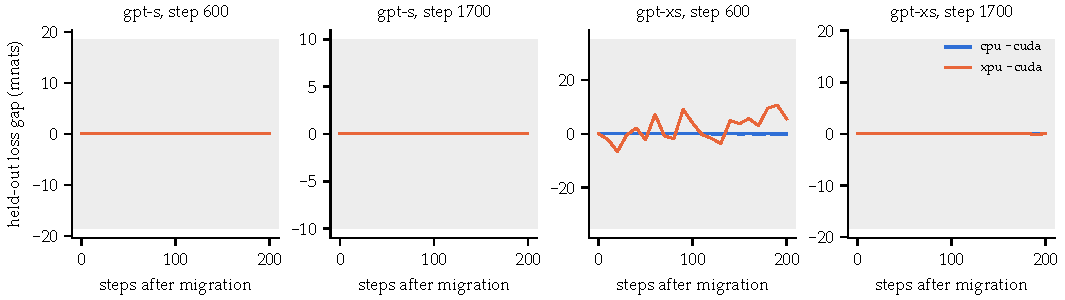
\includegraphics[width=0.95\textwidth]{device}
\caption{Held-out loss gap between devices after resuming the same full payload.}
\label{fig:device}
\end{figure*}

\section{The Larger Model}

Table~\ref{tab:large} gives the \largeParams{}M-parameter model in the format of the main table: \largeSeeds{} seeds,
migrations at 10\% and 60\% of the schedule, five strategies.

\begin{table*}[!htb]
\caption{Cost of each strategy on the \largeParams{}M-parameter model. Columns as in the main table.}
\label{tab:large}
\centering
\footnotesize
\begin{fit}\begin{tabular}{@{}lrrrrrccc@{}}
\toprule
Strategy & Payload\,\% & Peak (mnats) & Peak/$\eps$ & Regret (nat-steps) & Steps lost & StR\,$=0$ & StR & $>\!W$ \\
\midrule
\gen{tab_large}
\bottomrule
\end{tabular}\end{fit}
\end{table*}

\section{Preemption and Resizing with Multiple Ranks}

Table~\ref{tab:resize} repeats the end-to-end experiment of the main text with CPU ranks on one host, changing the number
of ranks at each preemption: two ranks shrink to one, and a later preemption grows the job back to two. The run
ended with a held-out loss \chaosResizeGap{} mnats from the uninterrupted run, and mean time to recovery was
\chaosResizeMttr\,s. It took \chaosResizeWall\,s of wall-clock time against \chaosResizeWallCtrl\,s for its control,
so the cost of the three interruptions is below the timing noise of CPU runs on this machine.

\begin{table*}[!htb]
\caption{Injected preemptions and a crash with a change of world size (\paramsXS{}M parameters, CPU ranks on one host).
Times in seconds unless marked.}
\label{tab:resize}
\centering
\footnotesize
\begin{fit}\begin{tabular}{@{}lrlrrrrrrrr@{}}
\toprule
Event & Step & World & Steps redone & Payload (MB) & Drain & Restart & Init & Fetch (ms) & Rebuild (ms) & Downtime \\
\midrule
\gen{tab_chaos_resize}
\bottomrule
\end{tabular}\end{fit}
\end{table*}

\section{Reproduction}

\sloppy Each table and figure is rebuilt from the run directories by one command, \texttt{python scripts/paper.py}; the
experiments themselves are launched with \texttt{scripts/run\_experiment.py}, \texttt{scripts/xdevice.py},
\texttt{scripts/latency.py}, \texttt{scripts/trace.py}, \texttt{scripts/diagnose.py} and \texttt{scripts/chaos.py} and
the configuration files under \texttt{configs/experiments}. Every run directory holds a manifest with the commit, the
resolved configuration, the device and library versions, the measured payload size and the median step time.


\end{document}
